\section{Zielsetzung}
\label{sec:Zielsetzung}
In diesem Versuch sollen die Erscheinungen des Photoeffekts näher untersucht werden. Zuerst wird die Frequenz beziehungsweise die Wellenlänge des Lichtes und ihr Zusammenhang mit der Elektronenenergie untersucht, um die Austrittsarbeit $A_\text{K}$ und die Größe $\frac{h}{e_0}$ zu bestimmen.
Dann wird an einer beleuchteten Photozelle die Abhängigkeit des Elektronenstromes von der Spannung gemessen und der Kurvenverlauf erklärt.

\section{Theorie}
\label{sec:Theorie}
Der Photoeffekt beschreibt das Herauslösen von Elektronen aus einem Metall durch Photonen, also durch Bestrahlung mit Licht. Für die Erklärung des Photoeffekts und anderer physikalischen Erscheinungen muss von einer korpuskularen Theorie des Lichtes ausgegangen werden. 

Die klassische Physik ist hier nicht in der Lage eine Beschreibung des Lichtes zu liefern. Dafür gibt es die Quantenelektrodynamik, die in ihrer Theorie zwei Grenzfälle beinhaltet. Die eine ist die Wellentheorie, bei der über eine großen Anzahl von Photonen, den Lichtquanten, die räumliche Ausbreitung des Lichtes beschrieben werden kann. 
Geht es allerdings um Wechselwirkungen von Licht mit Materie, so wird der zweite Grenzfall, die Teilchentheorie, zur Beschreibung genutzt. Diese Teilchen sind nach Einstein gleich mit den Planckschen Energiequanten und die ersten Erklärungen zu den lichtelektrischen Effektes konnte Einstein abgeben.

\begin{figure}[h!]
	\centering
	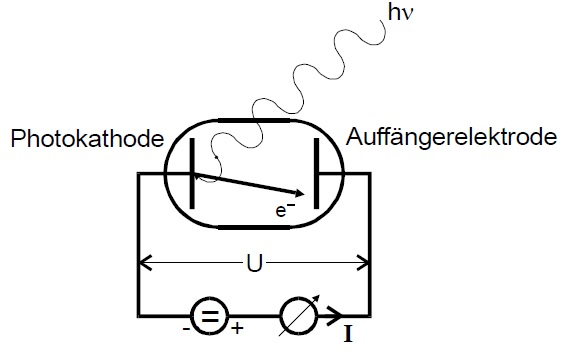
\includegraphics[width=0.6\linewidth]{AufbauPhotoeffekt.jpg}
	\caption{Schematischer Aufbau des Photoeffektes und dessen Untersuchung anhand der Bestrahlung des Materials mit monochromatischem Licht, \cite[2]{anleitung500}.}
	\label{fig:aufbauphotoeffekt}
\end{figure}

In der Abbildung \ref{fig:aufbauphotoeffekt} ist eine Vakuumaparatur zu sehen, in der die ausgelösten Elektronen aus elektrischer Strom nachgewiesen werden können. Das Material wird zuerst mit monochromatischem Licht bestrahlt. Dieser Elektrode, 
die negativ geladen ist, wird eine zweite gegenüber gestellt, die positiv geladen ist, so dass der elektrische Strom beobachtet werden kann. 
Bei der Durchführung dieses Experimentes wird zum einen die Beobachtung gemacht, dass die Energie der Elektronen proportional zur Lichtfrequenz und unabhängig von der Lichtintensität ist und zum anderen, dass es eine Grenzfrequenz gibt. 
Mit einem angepassten Versuchsaufbau könnte außerdem gezeigt werden, dass die Anzahl der ausgelösten Elektronen pro Zeitintervall proportional zur Lichtintensität sind.
Die Photonen, die sich mit der Lichtgeschwindigkeit $c$ bewegen, besitzen die Energie $h\nu$, wobei $h$ das Plancksche Wirkungsquantum ist. Die Energie $h\nu$ hängt somit von der Frequenz $\nu$ des Lichtes ab.
Um die Elektronen aus dem Metall herauszulösen, muss Arbeit verrichtet werden. Die Energie wird auf die Elektronen des Kathodenmaterials übertragen, damit sich das Elektron überhaupt lösen kann. Diese wird als Austrittsarbeit $A_\text{k}$ bezeichnet. 
Als wichtigste Beobachtung ist die maximale kinetische Energie $E_\text{max}$ zu nennen, die an das Elektron abgegeben wird. 
Als Energiebilanz ergibt sich:
\begin{equation}
\label{eq:eq1}
h \cdot \nu = E_\text{max} + A_\text{k}
\end{equation}
wobei $A_\text{k}$ die Austrittsarbeit ist und vom bestrahlten Material abhängt.
Aus der Gleichung \ref{eq:eq1} lässt sich erschließen, dass der Photoeffekt nicht mehr eintreten kann, wenn
\begin{equation*}
h \nu < A_\text{k}
\end{equation*}
gilt, weil dann keine Elektronen mehr ausgelöst werden können. 

\section{Experimentelle Untersuchung des Photoeffektes}
\begin{figure}[h!]
	\centering
	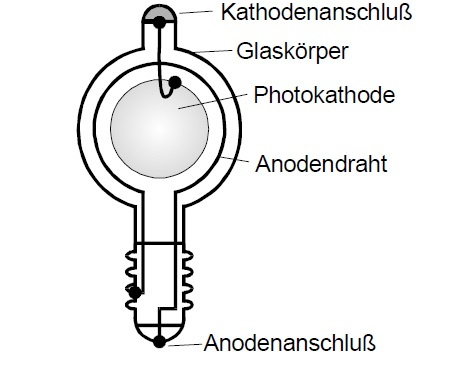
\includegraphics[width=0.5\linewidth]{AufbauPhotozelle.jpg}
	\caption{Aufbau einer Photozelle, \cite[4]{anleitung500}.}
	\label{fig:aufbauphotozelle}
\end{figure}
In der Abbildung \ref{fig:aufbauphotozelle} ist der schematische Aufbau einer Photozelle zu sehen. Zu sehen ist ein evakuierter Glaskörper, welcher zwei Elektroden enthält. Zum einen besteht die Photokathode aus einer Metall- oder Legierungsschicht, die vom Licht bestrahlt werden kann und zum anderen wird bei der Anode ein Drahtring verwendet, sodass er nah an der Kathode vorbeiführen kann.

\begin{figure}[h!]
	\centering
	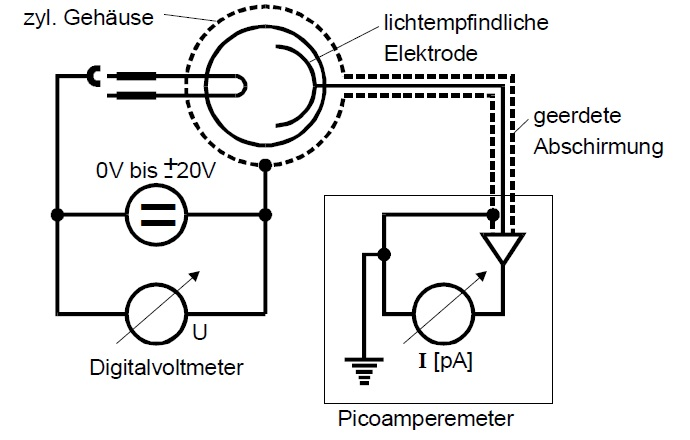
\includegraphics[width=0.7\linewidth]{ElektrischesSchaltbild.jpg}
	\caption{Elektrische Verbindung der Photozelle, \cite[5]{anleitung500}.}
	\label{fig:elektrischesschaltbild}
\end{figure}

In der Abbildung \ref{fig:elektrischesschaltbild} wird mit Hilfe der Gegenmethode die Energie des ausgelösten Elektronen untersucht. Die beiden Elektroden werden, wie in der Abbildung \ref{fig:elektrischesschaltbild} zu sehen ist, über ein Potential $U$ angelegt. Der Strom beginnt von der Kathode bis zur Anode an zu fließen. Es erreichen nur die Elektronen zur Anode, deren Energie größer ist als $e_0U$.
Der Strom verschwindet erst wenn:
\begin{equation}
\label{eq:eq2}
e_0U_\text{g} = \frac{1}{2}m_0v_\text{max}^2
\end{equation}
gilt, wobei $m_0$ die Masse des Elektrons, $e_0$ die Elementarladung und $v_\text{max}$ die Geschwindigkeit der schnellsten Elektronen sind. Die Energie der schnellsten Elektronen lassen sich mit der Hilfe der Gleichungen \ref{eq:eq1} und \ref{eq:eq2} bestimmen und in der folgenden Form umschreiben:
\begin{equation}
\label{eq:eq3}
h\nu = e_0U + A_\text{k}.
\end{equation}
Der Photostrom in Abhängigkeit von der Bremsspannung nimmt immer mehr ab, solange $U < U_\text{g}$ gilt. Der Verlauf ist in der Abbildung \ref{fig:photostrom} zu sehen. 
\begin{figure}[h!]
	\centering
	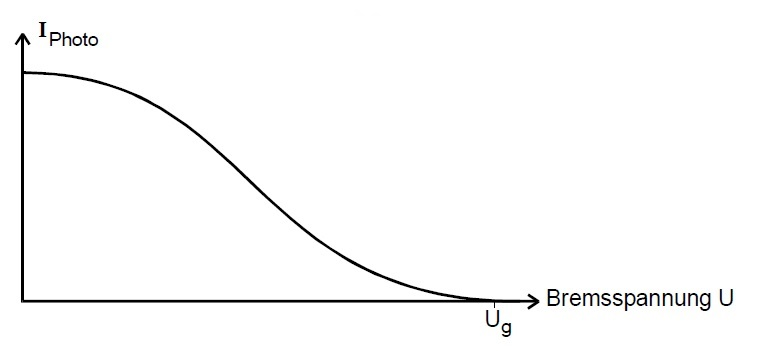
\includegraphics[width=0.7\linewidth]{Photostrom.jpg}
	\caption{Verlauf des Photostroms in Abhängigkeit der Bremsspannung, \cite[6]{anleitung500}.}
	\label{fig:photostrom}
\end{figure}
Dies lässt sich dadurch erklären, dass die Photoelektronen alle unterschiedliche Geschwindigkeiten zwischen $0$ und $\frac{1}{2}m_0v_\text{max}^2$ besitzen, weil sie unterschiedliche Energien besitzen. Über diese Energie gibt es die Fermi-Dirac-Statistik, die besagt, dass die Energie der Elektronen in einem Intervall von $0$ bis $\zeta$ liegt, wobei $\zeta$ die Fermi-Energie ist und je nach Material mehrere $\si{\electronvolt}$ betragen kann. 
Unter bestimmter Voraussetzungen ergibt sich ein parabolischer Zusammenhang zwischen dem Photostrom $I_\text{ph}$ und Bremsspannung $U$:
\begin{equation*}
I_\text{ph} \propto U^2.
\end{equation*}
Es gibt auch den Fall, dass der Photostrom nicht auftreten kann, wenn die Austrittsarbeit der Anode $A_\text{a}$ höher ist als $h \nu$. Dann müssten die Elektronen gegen ein Gegenfeld anlaufen, um die Anode zu erreichen. Es wird erst dann ein Photostrom beobachtet, wenn ein Potential angelegt wird, sodass:
\begin{equation*}
h \nu + e_0U_b \geq A_\text{a}
\end{equation*}
gilt, wobei $U_b$ ein beschleunigendes Potential ist. 